%  -----------------------------------------------------------------------------
%  Author         : Bimalka Piyaruwan Thalagala
%  GitHub         : https://github.com/bimalka98
%  Date Created   : 01.09.2020
%  Last Modified  : 18.02.2020
%  -----------------------------------------------------------------------------

\documentclass[a4paper,11pt]{article}%,twocolumn
\input{settings/packages}
\input{settings/page}
\input{settings/macros}


\begin{document}

\begin{titlepage}
\center % Center everything on the page

%-------------------------------------------------------------------------------------
%	HEADING SECTIONS
%------------------------------------------------------------------------------------
\textbf{\large Department of Electronic and Telecommunication Engineering}\\[0.5cm]
\textbf{\Large University of Moratuwa, Sri Lanka}\\[1cm]
\textbf{\large MA2033 - Linear Algebra}\\[2cm]
\includegraphics[width=0.3\textwidth]{figures/uomlogo}\\[2cm]

	
%-------------------------------------------------------------------------------------
%	TITLE SECTION
%------------------------------------------------------------------------------------
\textbf{\Huge Applications of Linear Algebra}\\[5mm]
\textbf{\Large Project Report}


%----------------------------------------------------------------------------------------
%	MEMBERS SECTION
%----------------------------------------------------------------------------------------

\vfill

\textbf{\large Submitted by}\\[0.5cm]

{\large Thalagala B.P.}	\hspace{5mm} {\large 180631J }\\[1cm]

%----------------------------------------------------------------------------------------
%	DATE SECTION
%----------------------------------------------------------------------------------------

\textbf{\large Submitted on}\\[0.5cm]
\textbf{\Large \today} % Date, change the \today to a set date if you want to be precise

%----------------------------------------------------------------------------------------


\end{titlepage}
\tableofcontents

\begin{center}
	\textbf{\textit{* PDF is clickable}}
\end{center}
\vspace{1cm}
\hrule


%%-----------------------------------------------------------------------


\section{Computer Vision: Detecting Corners/Features of an Image}

\textit{\large \textbf{Related Concepts in Linear Algebra:} Eigenvalues, Eigenvectors, Characteristic Polynomial, Quadratic Forms, Principal Axis Theorem, Orthogonal matrix, Diagonalization}

\subsection{Problem Identification}

In computer vision field finding corners/features in an image($I(x, y)$) is a key operation which is done prior to many advanced applications such as feature mapping, panorama stitching and 3D reconstruction. A corner can be identified as a point in an image whose neighborhood is locally unique to the given image. When comparing this neighborhood with any of the surrounding neighborhoods, significant difference can be observed between them.\\

This difference can be quantified mathematically using the following function evaluated over a region called a window($W$). Here the most basic Error function is used to make the explanation easy, and this may vary in different implementation of corner detection algorithms.

\begin{equation}
	E(u,v) = \sum_{(x,y) \in W}[I(x+u, y+v) – I(x, y)]^2
\end{equation}

This function can be further simplified using Taylor series and can be rearranged to get an expression in the \textbf{\textit{Quadratic form associated with $M$}} where the $M$ is called the \textit{\textbf{Second Moment Matrix}} which consists of summation of quadratic forms of gradients of the image over a window centered at the point of interest. Here gradient of the image along x axis is $I_{x}$ while $I_{y}$ is the gradient along y axis.

\begin{equation}
	 \begin{split}
		 	E(u,v) &= \sum_{(x,y) \in W}[I_{x}^{2}.u^{2}+2.I_{x}.I_{y}.u.v + I_{y}^{2}.v^{2}]\\
		 	&= \begin{bmatrix} u & v \end{bmatrix}
		 	 \begin{bmatrix}
		 	 	\sum_{(x,y) \in W}[I_x ^2 ]& \sum_{(x,y) \in W}[I_x I_y]  \\ \sum_{(x,y) \in W}[I_x I_y]& \sum_{(x,y) \in W}[I_y ^2 ]
	 	 	\end{bmatrix}
		 	\begin{bmatrix} u \\ v \end{bmatrix}\\
		 	&=\begin{bmatrix} u & v \end{bmatrix}M\begin{bmatrix} u \\ v \end{bmatrix}\\
		 	E(\underline{x})&= \underline{x}^\top M \underline{x}
	 \end{split}
  \label{euv}
 \end{equation}

The plot of the above function looks like follows for a given point where the $\sum_{(x,y) \in W}[I_x ^2 ]= 105983042.0$, $\sum_{(x,y) \in W}[I_x I_y]=13718014.0$ and $\sum_{(x,y) \in W}[I_y ^2 ]=105671174.0$\cite{cv}. (\textit{These values correspond to an actual corner in the Figure \ref{corners}}). If the point of interest is a corner it will give a very large Error ($E(u,v)$) value even for a very low ($u,v$) shift in any direction. This can be intuitively recognized as a steep surface(more narrower bowl shape) as depicted in Figure \ref{euvsurf}.

\begin{figure}[!h]
	\centering
	\subfigure[Surface Plot of $E(u,v)$]
	{ \includegraphics[scale=0.67]{figures/euvsurf}
\label{euvsurf}
}\hfill
	\subfigure[Contour Plot(Horizontal Slices) of $E(u,v)$]
	{ 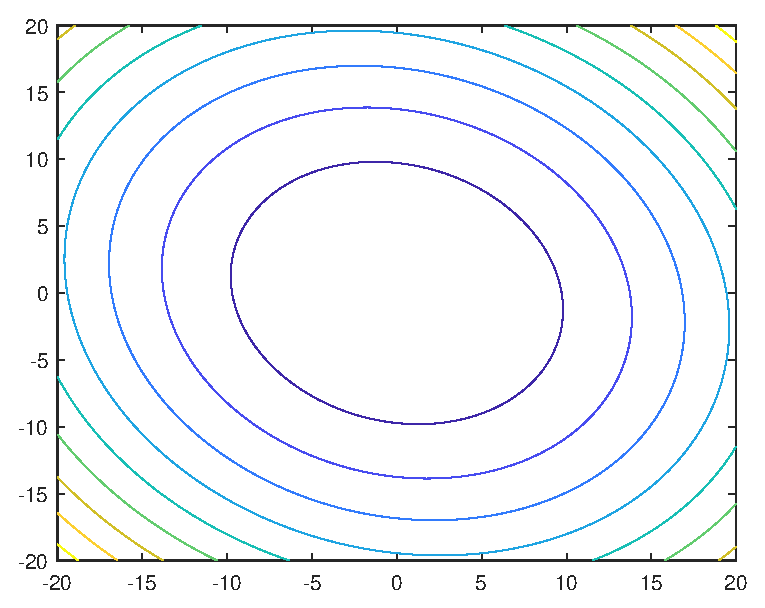
\includegraphics[scale=0.67]{figures/euvcontour}
\label{euvcontour}
}
	\caption{Error Function E(u,v) }

\end{figure}



\subsection{Solution through concepts of Linear Algebra}

This narrowness can be mathematically quantified by examining a horizontal slice of the surface plot in figure \ref{euvsurf}. Consider one particular contour in Figure \ref{euvcontour}, then along that contour, function value is a constant i.e $E(\underline{x}) = constant = \underline{x}^\top M \underline{x}$ and then the above Expression \ref{euv} represents equation of an ellipse. \textit{If the surface is narrow, the radii of the ellipse must be small for a given $E(u,v)$ value.} That is function value must increase rapidly as we moves outward from the point of interest. Lengths of the major and minor axes(radii) of the ellipse are given by $\lambda_{min}^{-\frac{1}{2}}$ and $\lambda_{max}^{-\frac{1}{2}}$ respectively, where the $\lambda_{min}$ and $\lambda_{max}$ are the \textbf{\textit{eigenvalues associated with the second moment matrix $M$}}. We can prove this as follows\cite{corner}.\\

Since $M$ is a symmetric matrix, an \textbf{\textit{Orthogonal($P^\top=P^{-1}$) matrix}} $P$ can be found such that $\underline{x} = P\underline{y}$  which transforms $E(\underline{x}) = \underline{x}^\top M \underline{x}$ into the form  $E(\underline{y}) = \underline{y}^\top D \underline{y}$ where $D$ is a diagonal matrix consists of the eigenvalues of the $M$. The columns of matrix $P$ consists of the \textbf{\textit{eigenvectors}} associated with the eigenvalues of the second moment matrix $M$.

\begin{equation}
	\begin{split}
E(\underline{x}) &= \underline{x}^\top M \underline{x}\\
&= (P\underline{y})^\top M (P\underline{y})\\
&= (\underline{y}^\top P^\top) M (P\underline{y})\\
&= \underline{y}^\top (P^\top M P)\underline{y}\\
&= \underline{y}^\top D \underline{y}\\
E({y_{1},y_{2}})&= \begin{bmatrix} y_{1} & y_{2} \end{bmatrix}
\begin{bmatrix}
	\lambda_{min} & 0  \\ 0 & \lambda_{max}
\end{bmatrix}
\begin{bmatrix} y_{1} \\ y_{2} \end{bmatrix}\\
	 \end{split}
 \label{orthdiag}
\end{equation}

Comparing result of Expression \ref{orthdiag} with the standard form of an ellipse,

\begin{equation}
	\begin{split}
		{\frac{x^2}{a^2} + \frac{y^2}{b^2}} &= {\begin{bmatrix} x & y \end{bmatrix}
		\begin{bmatrix} 1/a^2 & 0 \\ 0 & 1/b^2 \end{bmatrix}
		\begin{bmatrix} x \\ y \end{bmatrix}} \\
 &= {\begin{bmatrix} y_{1} & y_{2} \end{bmatrix}
		\begin{bmatrix}\lambda_{min} & 0  \\ 0 & \lambda_{max} \end{bmatrix}
		\begin{bmatrix} y_{1} \\ y_{2} \end{bmatrix}}\\
	\end{split}
\end{equation}

Therefore, $1/a^2 = \lambda_{min}$ and $1/b^2 = \lambda_{max}$. Which yields that
$a = \lambda_{min}^{-\frac{1}{2}}$ and $b = \lambda_{max}^{-\frac{1}{2}}$.\\

Therefore to find corners in an image all we have to do is find the \textbf{\textit{eigenvalues}} associated with each second moment matrix for each pixel$(x,y)$ in an image. According to the magnitudes of eigenvalues following classification can be done.

\begin{enumerate}[a.)]
	\item  \textbf{At a Corner:} $E(u,v)$ increases rapidly in any direction and therefore \textit{both eigenvalues are large}.
	\item 	\textbf{At an Edge:}  $E(u,v)$ increases rapidly only in one direction and therefore \textit{one eigenvalue is relatively larger than the other}.
	\item \textbf{At a flat area:} $E(u,v)$ does not increase rapidly and therefore \textit{both eigenvalues are small}.
\end{enumerate}


\begin{figure}[!h]
\centering
\includegraphics[scale= 0.3]{figures/corner}
\caption{Detecting corners in an image, Step by Step approach\cite{cv}}
\label{corners}
\end{figure}

Calculating eigenvalues is computationally expensive therefore what is known as Corner Response Function(R) is used when implementing algorithms. Here $\alpha$ $\in$ [0.04,0.06] and \textbf{At a Corner:} R $\gg$ 0, \textbf{At an Edge:} R $<$ 0, \textbf{At a flat area:} $|R|$ is small. Therefore corners can be extracted by applying an appropriate threshold value for R.

\begin{equation}
	\begin{split}
R &= det(M) - \alpha* trace(M)^2\\
 & = \lambda_{min}*\lambda_{max} - \alpha*(\lambda_{max} + \lambda_{min})^2
	\end{split}
\end{equation}




\pagebreak

\section{Robotic Systems: Coordinate frame Transformation}

\textit{\large \textbf{Related Concepts in Linear Algebra:} Linear Transformations, Matrix Transformations, Change of basis, Matrix Multiplication}

\subsection{Problem Identification}

When robot arms are used in industrial activities, robot engineer needs to make sure the \textbf{\textit{end-effector}}(\textit{gripper or any other tool attached at the end of the arm}) of the robot arm is at the exact location in the exact orientation at the operation. Otherwise the required behavior of the arm can not be obtained. Problem is usually robot takes the measurements using sensors or cameras placed somewhere else in the system and therefore these measurements(\textbf{\textit{position vectors}}) are in with respect to those sensor's or camera's coordinate frame while the robot arm operates with respect to some other(Robot base) coordinate frame. Flowing figure illustrates this situation.\\

\begin{figure}[!h]
	\centering
	\subfigure[Robotic System]
	{ \includegraphics[scale=0.67]{figures/env}		
	}\hfill
	\subfigure[Coordinate Systems]
	{ \includegraphics[scale=0.67]{figures/difcord}		
	}
	\caption{Use of Different Coordinate systems in an Industrial Robotic System\cite{pics}}	
\end{figure}

Therefore to make use of the information gathered by the sensors/cameras first we need to \textbf{\textit{transform}} position vectors gathered by camera with respect to its coordinate frame, in to robot arm's base coordinate frame. Then we can use inverse kinematics to calculate the required rotation angles and translations that we should provide to the arm to get the required behavior. 

\subsection{Solution through concepts of Linear Algebra}

In order to fully describe an object in the 3D world we need its \textit{\textbf{Rotation and Translation}} with respect to some reference(\textit{in this case the robot arm}) coordinate frame(say $\alpha$). For that the object of interest(\textit{in this case the sensor/camera}) must be given its own coordinate frame(say $\beta$) too. The mathematical way to represent differences between the reference frame and the object's frame is called the \textbf{\textit{Homogeneous Transformation Matrix}}\cite{robotic} in Robotics and it is denoted as,

\begin{center}
	$ H^{\alpha}_{\beta} $ : read as transformation of frame $\beta$ with respect to the frame $\alpha$
\end{center}

This 	$ H^{\alpha}_{\beta} $ can be mathematically represented as a $4 \times 4$ matrix which consists of $3 \times 3$ Rotation matrix and a $3 \times 1$ Translation matrix with last row as $[0~0~0~1]$ to make it  $4 \times 4$ square matrix to make the computation easy.

\begin{equation}
	\begin{split}
		 H^{\alpha}_{\beta} &=
			\begin{bmatrix}
				 r_{11} & r_{12} & r_{13} & d_1 \\
				 r_{21} & r_{22} & r_{23} & d_2 \\
				 r_{31} & r_{32} & r_{33} & d_3 \\
				 0 & 0 & 0 &1 \\
			\end{bmatrix}
	\end{split}
\end{equation}

There are  \textbf{\textit{6 Principal Movements}} as, rotations about 3 axes(X,Y,Z) and translations along 3 axes(X,Y,Z). Correct combination(\textit{obtain by multiplying required principal matrices like $Rot(e_i,\theta_m)*Trans(e_j,d_k)$}) of these 6 principal movements  can be used to get any of the advanced transformations, from the reference frame to object's frame. Those basic matrices are as follows where $e_i$ refers to the elements in standard \textbf{\textit{basis}}( $e_1 = [1 ~0~ 0]^\top$, $e_2 = [0 ~1~ 0]^\top$ and $e_3 = [0 ~0~ 1]^\top$) while $\theta_i$ indicates how many degrees the object has rotated about the $e_i$ basis vector. Additionally $d_i$ indicates the displacement along the direction of $e_i$ basis vector(axis)\cite{tfs1}. \\

\begin{center}
	\begin{tabular}{| c || c|}
		\hline
 \textbf{Principal Rotations about axes(X,Y,Z)\cite{tfs2}} &	\textbf{Principal Translations along axes(X,Y,Z)\cite{tfs2}}\\\hline
 		&\\
		$Rot(e_1,\theta_1) =
\begin{bmatrix}
	1 & 0 & 0 & 0 \\
	0 & \cos(\theta_1) & -\sin(\theta_1) & 0 \\
	0 & \sin(\theta_1) & \cos(\theta_1) & 0 \\
	0 & 0 & 0 &1 \\
\end{bmatrix}$ & 
		$Trans(e_1,d_1)=
\begin{bmatrix}
	1 & 0 &0  & d_1 \\
	0 & 1 & 0 & 0 \\
	0 & 0 & 1 & 0 \\
	0 & 0 &0  & 1 \\
\end{bmatrix}$
\\[1cm]
%--------------------------------------------------------------------------
$Rot(e_2,\theta_1) =
\begin{bmatrix}
\cos(\theta_1)	& 0 & \sin(\theta_1)  & 0 \\
0	& 1 & 0 & 0 \\
-\sin(\theta_1)	& 0 & \cos(\theta_1) & 0 \\
0 & 0 & 0 &1 \\
\end{bmatrix}$ & 
		$Trans(e_2,d_2) =
\begin{bmatrix}
	1 & 0 &0  & 0 \\
	0 & 1 & 0 & d_2 \\
	0 & 0 & 1 & 0 \\
	0 & 0 & 0 & 1 \\
\end{bmatrix}$
\\[1cm]
%--------------------------------------------------------------------------
$Rot(e_3,\theta_1) =
\begin{bmatrix}
	\cos(\theta_1) & -\sin(\theta_1)&0  & 0 \\
	\sin(\theta_1) & \cos(\theta_1)   &0  & 0 \\
	0&0  &1  & 0 \\
	0 & 0 & 0 &1 \\
\end{bmatrix}$ & 
		$Trans(e_3,d_3) =
\begin{bmatrix}
	1 & 0 &0  & 0 \\
	0 & 1 & 0 & 0 \\
	0 & 0 & 1 & d_3 \\ 
	0 & 0 & 0 & 1 \\
\end{bmatrix}$\\
		&\\\hline\hline
\end{tabular}
\end{center}

Once we construct the \textbf{\textit{Homogeneous Transformation Matrix which transforms robot base frame  into camera frame}}, we just have to multiply the position vectors obtained w.r.t camera frame by this transformation matrix to get the corresponding position vectors in the robot base frame. Let  $^1u = [u_1 ~u_2~ u_3~1]^\top$ be a  position vector(homogeneous) of an object in the camera frame and  $H^{0}_{1}$ be the homogeneous transformation matrix, then the position vector of the object in the robot base frame is\cite{tfs3}, say $^0u$

\begin{equation}
	\begin{split}
		^0u &= H^{0}_{1}* ^1u\\
		^0u &=
		{\begin{bmatrix}
			r_{11} & r_{12} & r_{13} & d_1 \\
			r_{21} & r_{22} & r_{23} & d_2 \\
			r_{31} & r_{32} & r_{33} & d_3 \\
			0 & 0 & 0 &1 \\
		\end{bmatrix}} * \begin{bmatrix} u_1 \\u_2\\ u_3\\1 \end{bmatrix}
	\end{split}
\end{equation}

Moreover, since the Homogeneous Transformation Matrix is invertible, following expression is also valid which makes it possible to move between coordinate systems easily.
\begin{equation}
{H^{0}_{1}}^{-1} = H^{1}_{0}
\end{equation}

\vfill
\vspace{1cm}
\hrule

\scriptsize
\begin{flushleft}
	\bibliographystyle{plain}
\bibliography{refer}
\end{flushleft}
\end{document}
